% !TEX root = ../thesis.tex
\chapter{Related Work}

\label{ch:related-work}

\section{Similar systems and inspiration}

\subsection{Haxl}

Haxl\cite{Haxl:library:link}\cite{Marlow:2014:NFA:2692915.2628144} is a Haskell\cite{HaskellLanguage} library which provides a framework for performing data access operations with automatic batching and concurrency. It was first introduced in the paper ``There is No Fork: An Abstraction for Efficient, Concurrent, and Concise Data Access''\cite{Marlow:2014:NFA:2692915.2628144} by Simon Marlow, Louis Brandy, Jonathan Coens and Jon Purdy.

They describe a system where, by using the Haskell abstraction of an Applicative Functor\cite{mcbride2008applicative}, they are able to find which data access operations are independent from one another and therefore may be fetched as a batch job.

As a very small example in Figure~\ref{fig:operation-in-haxl} we see a function \texttt{commonFriends}.
The \texttt{intersection} function depends for its input on both the result of fetching the friends of \texttt{a} as well as the friends of \texttt{b}.
However the two data fetches \texttt{friendsOf a} and \texttt{friendsOf b} are independent from one another, neither depends on the result of the other, which is what the \texttt{<*>} operator symbolises.

\begin{figure}[h]
\begin{minted}{Haskell}
commonFriends a b =
    pure intersection
        <*> friendsOf a
        <*> friendsOf b
\end{minted}
\caption{An operation in Haxl}
\label{fig:operation-in-haxl}
\end{figure}

A program written with Haxl runs all independent program graphs blocking once it encounters a fetching operation.
When all program paths are either finished or blocking all the blocking requests are executed in what is called a `round'.
After the round finishes executing and the results are present the paths are resumed.
A very simple example can be seen in Figure~\ref{fig:haxl-basic-example}.
Additionally all requests are cached for a run of the Haxl program.

In the paper ``Ÿauhau: Concise Code and Efficient I/O Straight from Dataflow.''~\cite{ErtelGoensAdamEtAl2016} we criticise how the benefits of the Haxl framework require use of special functor operations, such as lifting the \texttt{intersection} operation into the Functor with \texttt{pure} and applying the arguments with \texttt{<*>}.
It is much more difficult writing this kind of code than the obvious and straight forward monadic code from Figure~\ref{fig:monadic-common-friends}.
For small examples adopting this alternative style is not as difficult, but as programs gets larger and more complicated the complexity of maintaining this particular style of writing code increases.

\begin{figure}[h]
\begin{minted}{Haskell}
commonFriends a b = do
    fa <- friendsOf a
    fb <- friendsOf b
    return (fa `intersection` fb)
\end{minted}
\caption{Monadic version of \texttt{commonFriends}}
\label{fig:monadic-common-friends}
\end{figure}

\begin{figure}
\begin{minted}{Haskell}
main =
    pure compute
        <*> fetch (increment 23)
        <*> fetch (42 + 1337)
        <*> fetch (log_e 2.71828 + 1337)
\end{minted}
    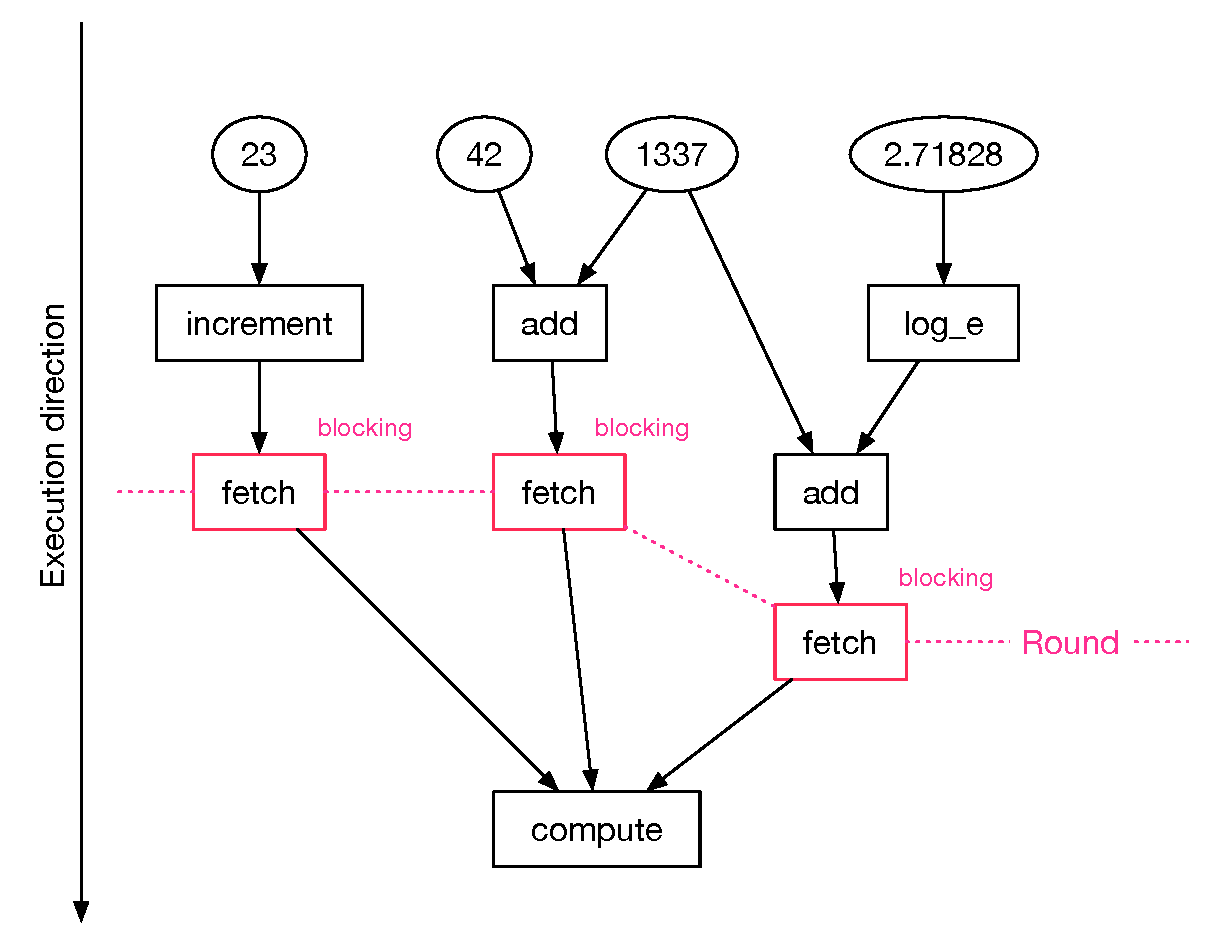
\includegraphics[width=\linewidth]{../Figures/haxl-basic-example}
    \caption{A visual example of the haxl execution}
    \label{fig:haxl-basic-example}
\end{figure}

\subsection{Muse}

Muse\cite{Muse:repository:link} is a Clojure implementation of Haxl.
Like Haxl the data access actions are defined with functors.
This functor is a free monad\cite{free-monad} which builds an AST of the program.
A runtime traverses that AST, finds parallel rounds of fetches and executes the code, batching the fetch operations.

\subsection{Datasources}

\label{subs:datasources}

Datasources can be arbitrary user defined targets for I/O actions such as databases, network requests or filesystem I/O.
However datasources must be defined separately and only for those defined datasources the optimisation can be leveraged.

Defining a datasource in Haxl means defining a set of actions on the source in form of a GADT\cite{PeytonJones:2006:SUT:1160074.1159811}, see Figure~\ref{fig:defining-requests-in-haxl} .

\begin{figure}
\begin{minted}{Haskell}
data FacebookRequest a where
    GetFriends :: UserID -> FacebookRequest [UserID]
    GetProfile :: UserID -> FacebookRequest Profile
\end{minted}
\caption{Defining requests in Haskell}
\label{fig:defining-requests-in-haxl}
\end{figure}


Every time you want to make a request in the program it has to be encoded into one of those actions.
A Haxl function by the name of \texttt{dataFetch} can be called with an encoded request to schedule its execution.

The actual execution of the I/O action is defined in a typeclass\cite{type-classes} called \texttt{DataSource} which has to be defined on the request GADT, see Figure~\ref{fig:defining-datsource-in-haxl}.
The \texttt{DataSource} typeclass has a method called \texttt{fetch} which does the actual work of performing the desired I/O action and is user defined.
Even though it allows arbitrary side effects due to the fact that Haxl caches results it is strongly recommended not to mutate the data source but only retrieve data.
As its type signature \texttt{fetch} method indicates, see  Figure~\ref{fig:defining-datsource-in-haxl}, it performs multiple requests simultaneously and this is where the batching happens.
The user defines how exactly these requests are batched, Haxl only concerns itself with finding requests that can be batched.

Additionally, for the cache, the \texttt{Hashable} typeclass needs to be implemented on this type as well as the \texttt{DataSourceName} and \texttt{StateKey} typeclass to identify the source.

\begin{figure}
\begin{minted}{Haskell}
class DataSource u request where
    fetch :: ... -> [BlockedFetch request] -> PerformFetch
\end{minted}
\caption{Defining a data source in Haxl}
\label{fig:defining-datsource-in-haxl}
\end{figure}

When the framework executes the actions each datasources gets all the requests for that particular datasource. Therefore all actions which can be batched together should be defined on the same datasource (in the same GADT) and actions which cannot be batched should be defined on separate datasources.

\section{Control flow}

Both Haxl and Muse use runtime data structures to aggregate fetch rounds.
In Haxl this is a \texttt{Data.Sequence.Seq}, which is a type of list.
At runtime, if a data fetch is encountered it simply gets appended to this list of fetches to execute.
This way Haxl builds a dynamic list of fetches to execute for each round each time the program is run.

This makes it easily to handle cases where the amount of fetches is not known at compile time.
For instance in conditionals or when executing a fetch over a collection, see Figure~\ref{fig:control-flow-in-haxl}.

\begin{figure}
\begin{minted}{Haskell}
mappedFetches = mapM fetch [a, b, ..]
-- -> [Request a, Request b, ..]

conditionalFetches execute =
    if execute
        then fetch 0 -- -> [Request 0]
        else return () -- -> []
\end{minted}
\caption{Control flow in Haxl}
\label{fig:control-flow-in-haxl}
\end{figure}

\section{Side effects}

\subsection{Haxl}

Both Haxl and Muse make very strict assumptions about the immutability of their programs.
In the case of Haxl side effects of any kind are prohibited.
A Haxl computation cannot access the Network or Hard drive, only pure actions, or Haxl data fetches are allowed.
This is enforced via the type system.
Furthermore Haxl strongly recommends that data fetches not perform mutative operations on the data source.
This is mainly because additionally to batching requests requests are also cached and when executed again are simply served from the cache.
A sequence of actions like Figure~\ref{fig:haxl-invalid-actions} would yield \texttt{False} in every case, since the second fetch of \texttt{a} would be served from the cache.

\begin{figure}
\begin{minted}{Haskell}
data Request = Retrieve Int | Mutate Int

invalid :: GenHaxl u Bool
invalid = do
    let a = ...
    data1 <- fetch (Retrieve a)
    fetch (Mutate a)
    data2 <- fetch (Retrieve a)
    return (data1 /= data2)
\end{minted}
\caption{Haxl invalid actions}
\label{fig:haxl-invalid-actions}
\end{figure}

\subsection{Muse}

Muse is more loose with its allowance of side effects, because in Clojure there is no type system which could be used to restrict I/O.
However it also caches previous requests and therefore the effects of mutating the data source are not reflected in future, cached fetches.
As a result muse also strongly recommends not to mutate the data source.
